% Native editable composition from verified, unchanged IDE images.
\par
\begin{figure}[htbp]
\centering
\sbox0{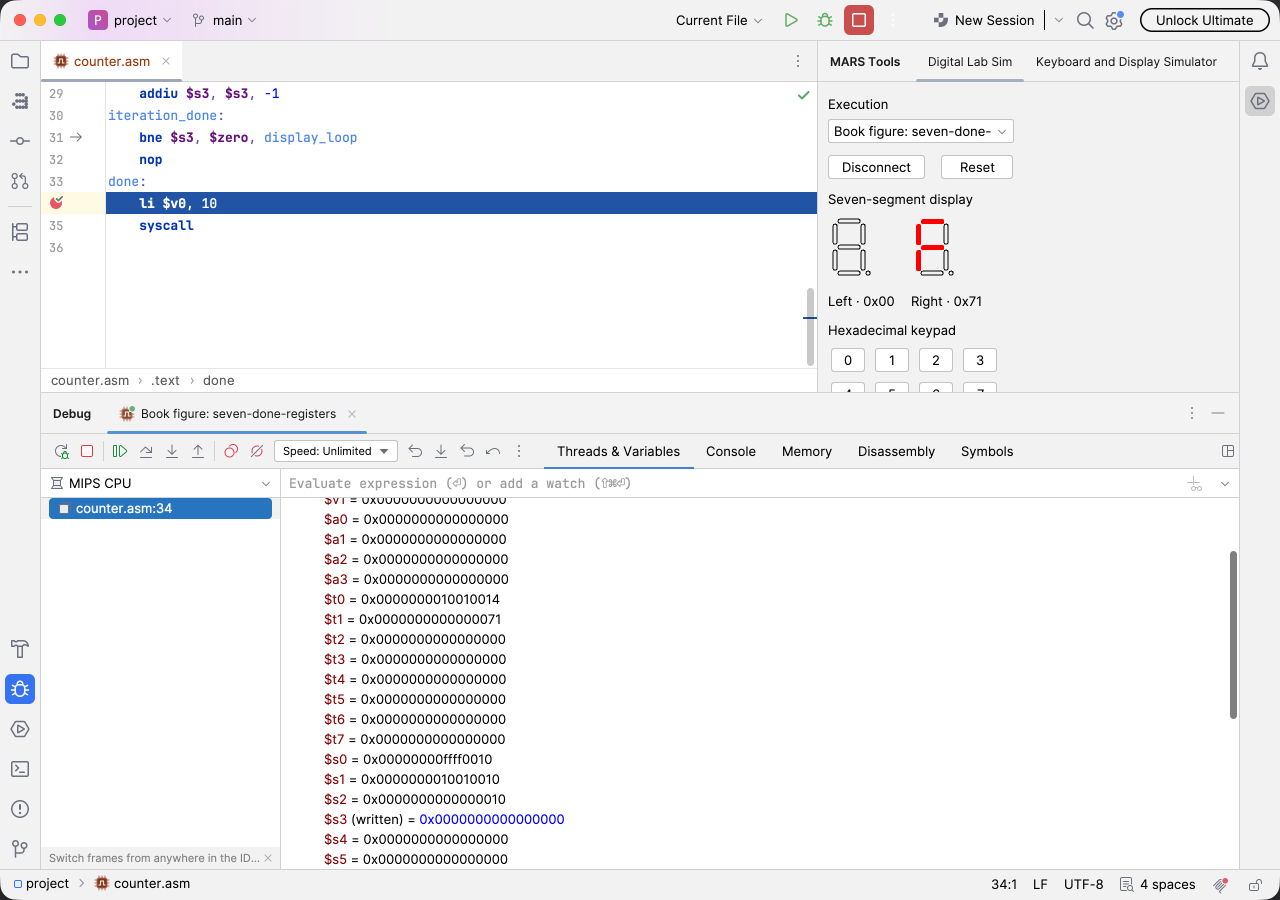
\includegraphics[artifact]{packages/005-seven-segment-counter/captures/f04-final-f/registers.png}}
\sbox2{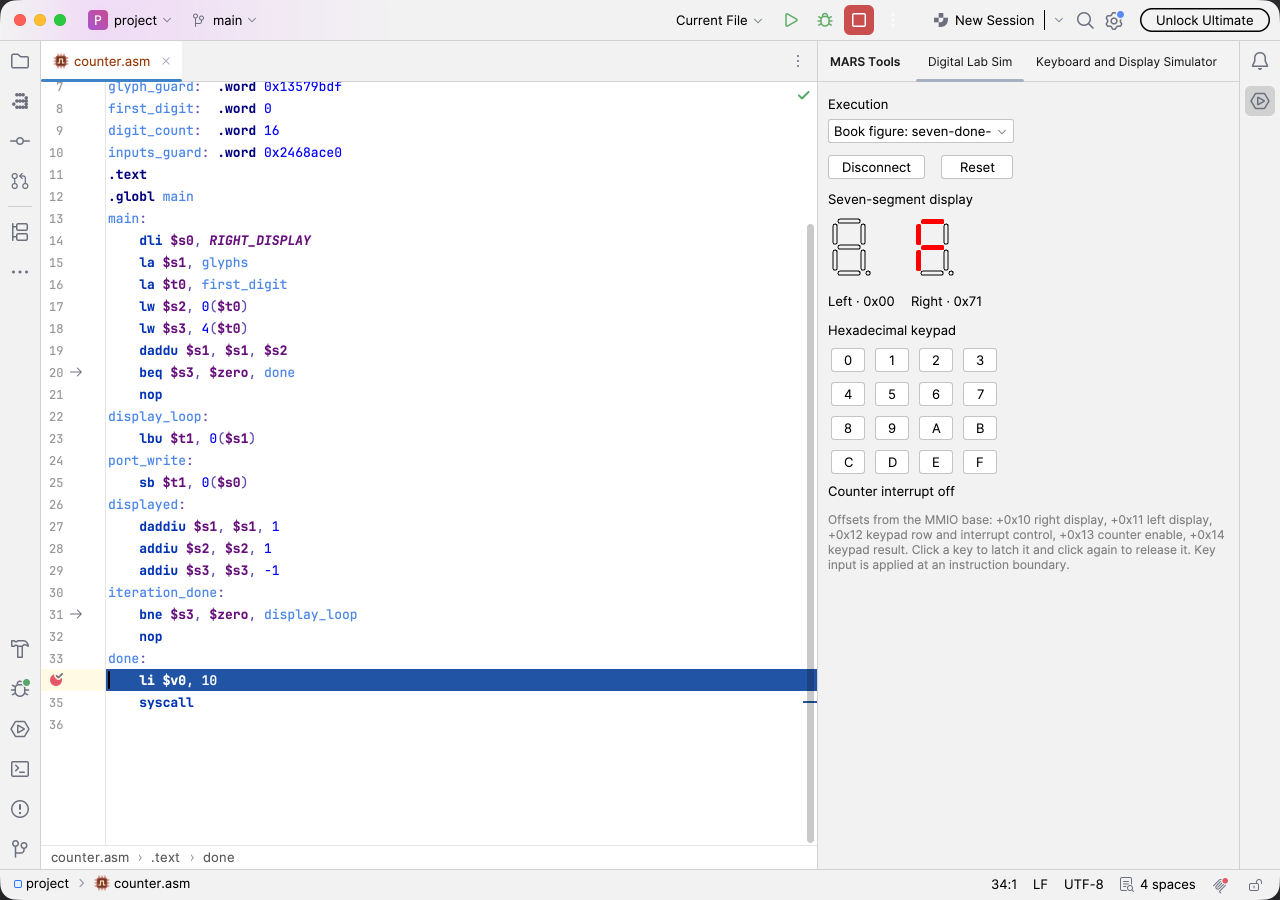
\includegraphics[artifact]{packages/005-seven-segment-counter/captures/f04-final-f/lab.png}}
\sbox4{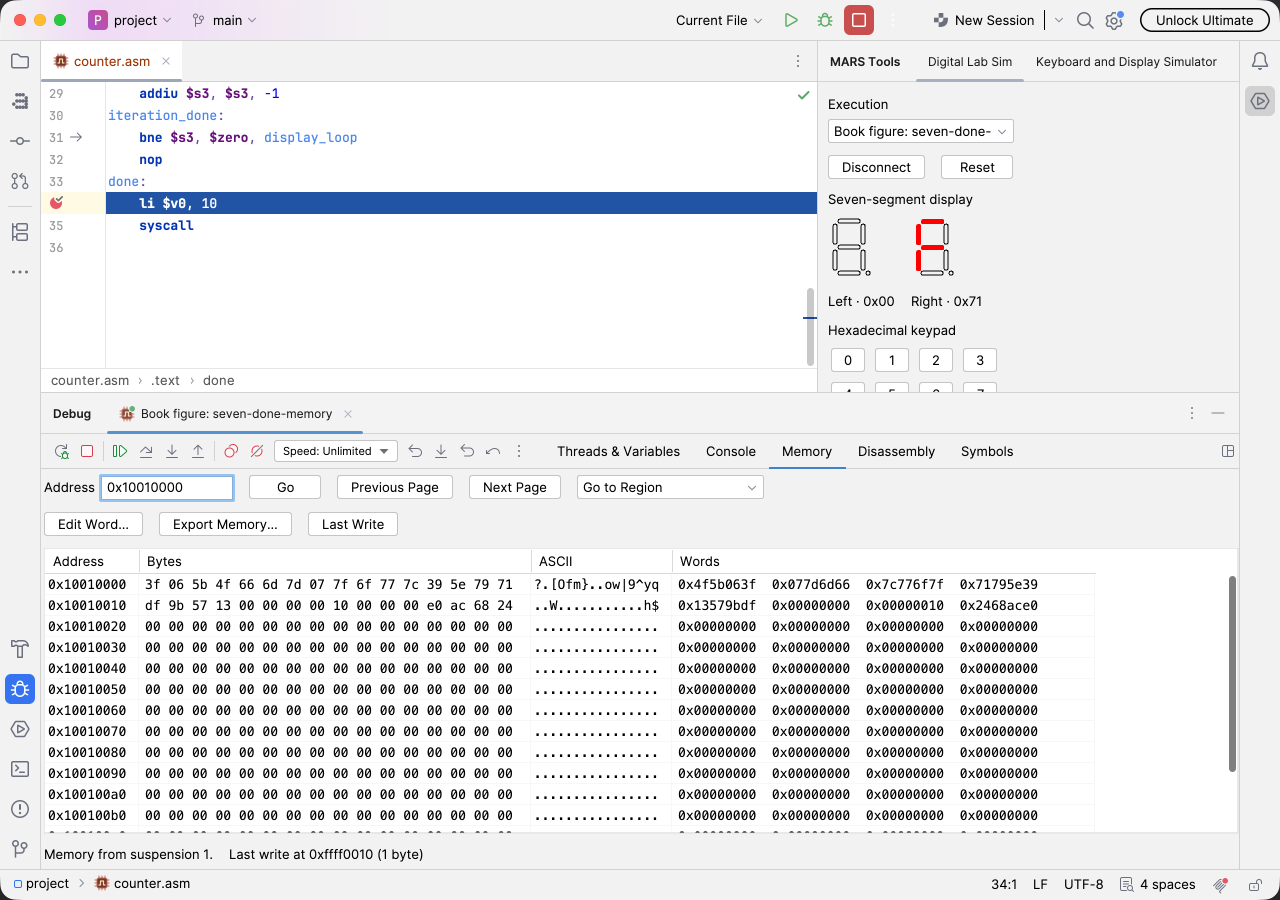
\includegraphics[artifact]{packages/005-seven-segment-counter/captures/f04-final-f/memory.png}}
\edef\MARSfinalsourceLeft{\the\dimexpr0.036718750\wd0\relax}
\edef\MARSfinalsourceBottom{\the\dimexpr0.757777778\ht0\relax}
\edef\MARSfinalsourceRight{\the\dimexpr0.611718750\wd0\relax}
\edef\MARSfinalsourceTop{\the\dimexpr0.164444444\ht0\relax}
\edef\MARSfinallabLeft{\the\dimexpr0.643750000\wd2\relax}
\edef\MARSfinallabBottom{\the\dimexpr0.652222222\ht2\relax}
\edef\MARSfinallabRight{\the\dimexpr0.228906250\wd2\relax}
\edef\MARSfinallabTop{\the\dimexpr0.213333333\ht2\relax}
\edef\MARSfinalregistersLeft{\the\dimexpr0.246093750\wd0\relax}
\edef\MARSfinalregistersBottom{\the\dimexpr0.075555556\ht0\relax}
\edef\MARSfinalregistersRight{\the\dimexpr0.553125000\wd0\relax}
\edef\MARSfinalregistersTop{\the\dimexpr0.873333333\ht0\relax}
\edef\MARSfinalmemoryLeft{\the\dimexpr0.034375000\wd4\relax}
\edef\MARSfinalmemoryBottom{\the\dimexpr0.311111111\ht4\relax}
\edef\MARSfinalmemoryRight{\the\dimexpr0.578906250\wd4\relax}
\edef\MARSfinalmemoryTop{\the\dimexpr0.608888889\ht4\relax}
\begin{tikzpicture}[alt={Four annotated details at done before li v0 ten. The right display retains F with mask 71 and the left remains blank. Register s2 is hexadecimal 10, meaning decimal sixteen, and s3 is zero. Two full memory rows retain the sixteen glyph bytes followed by the original guard, first index zero, count sixteen and trailing guard.}]
\node[anchor=north west,inner sep=0,font=\small\bfseries] (source-title) at (6mm,0) {The loop has reached its exit label};
\node[anchor=north west,inner sep=0] (source) at ([yshift=-1mm]source-title.south west) {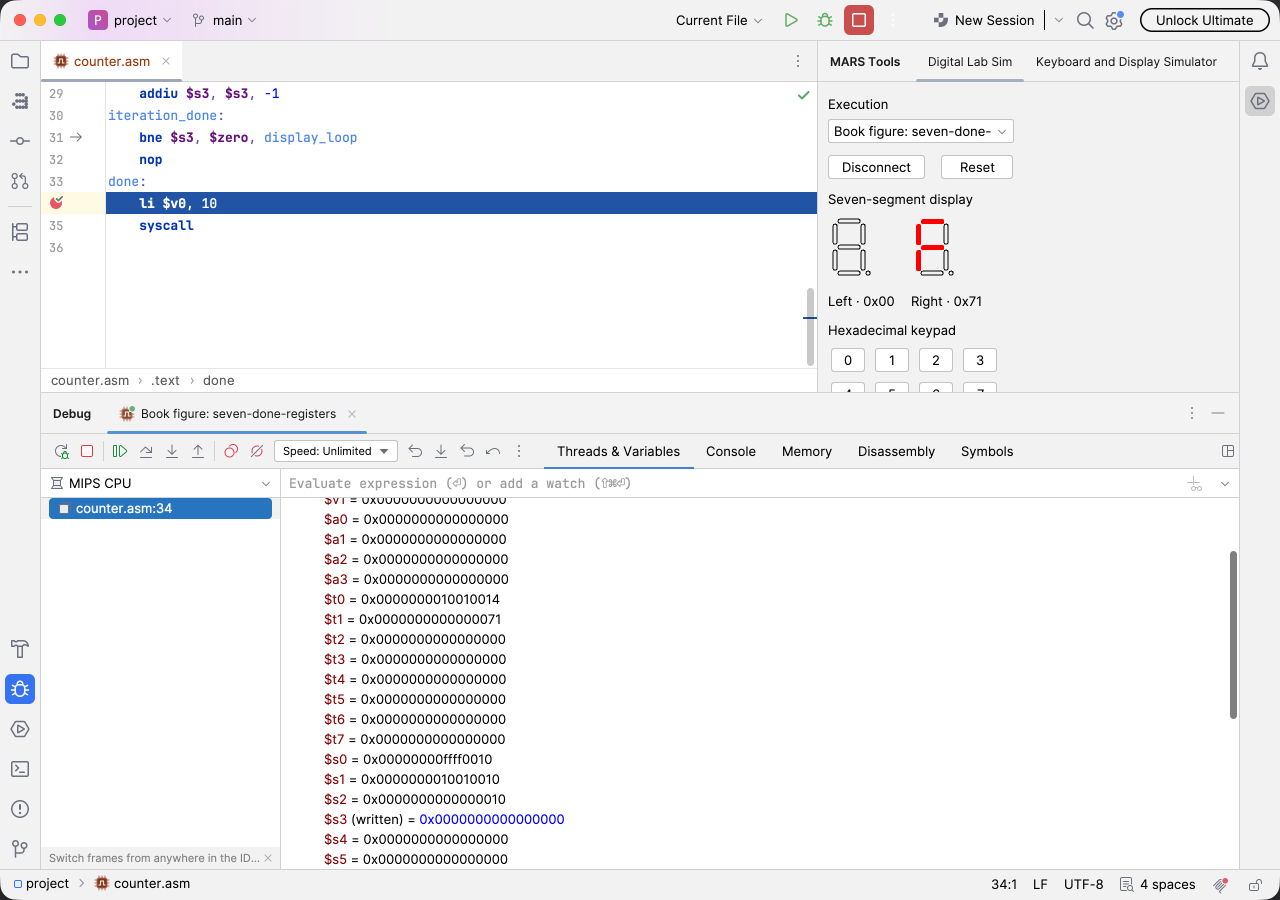
\includegraphics[width=0.7\linewidth,artifact,trim={\MARSfinalsourceLeft{} \MARSfinalsourceBottom{} \MARSfinalsourceRight{} \MARSfinalsourceTop{}},clip]{packages/005-seven-segment-counter/captures/f04-final-f/registers.png}};
\begin{scope}[shift={(source.south west)},x={($(source.south east)-(source.south west)$)},y={($(source.north west)-(source.south west)$)}]
\draw[black,line width=0.7pt] (0.135555556,0.057142857) rectangle (0.377777778,0.371428571);
\node[draw=black,fill=white,circle,inner sep=1.5pt,font=\footnotesize] at ($(0.135555556,0.371428571)+(-3mm,0)$) {1};
\end{scope}
\node[anchor=north west,inner sep=0,font=\small\bfseries] (lab-title) at ([yshift=-2mm]source.south west) {The last store remains visible};
\node[anchor=north west,inner sep=0] (lab) at ([yshift=-1mm]lab-title.south west) {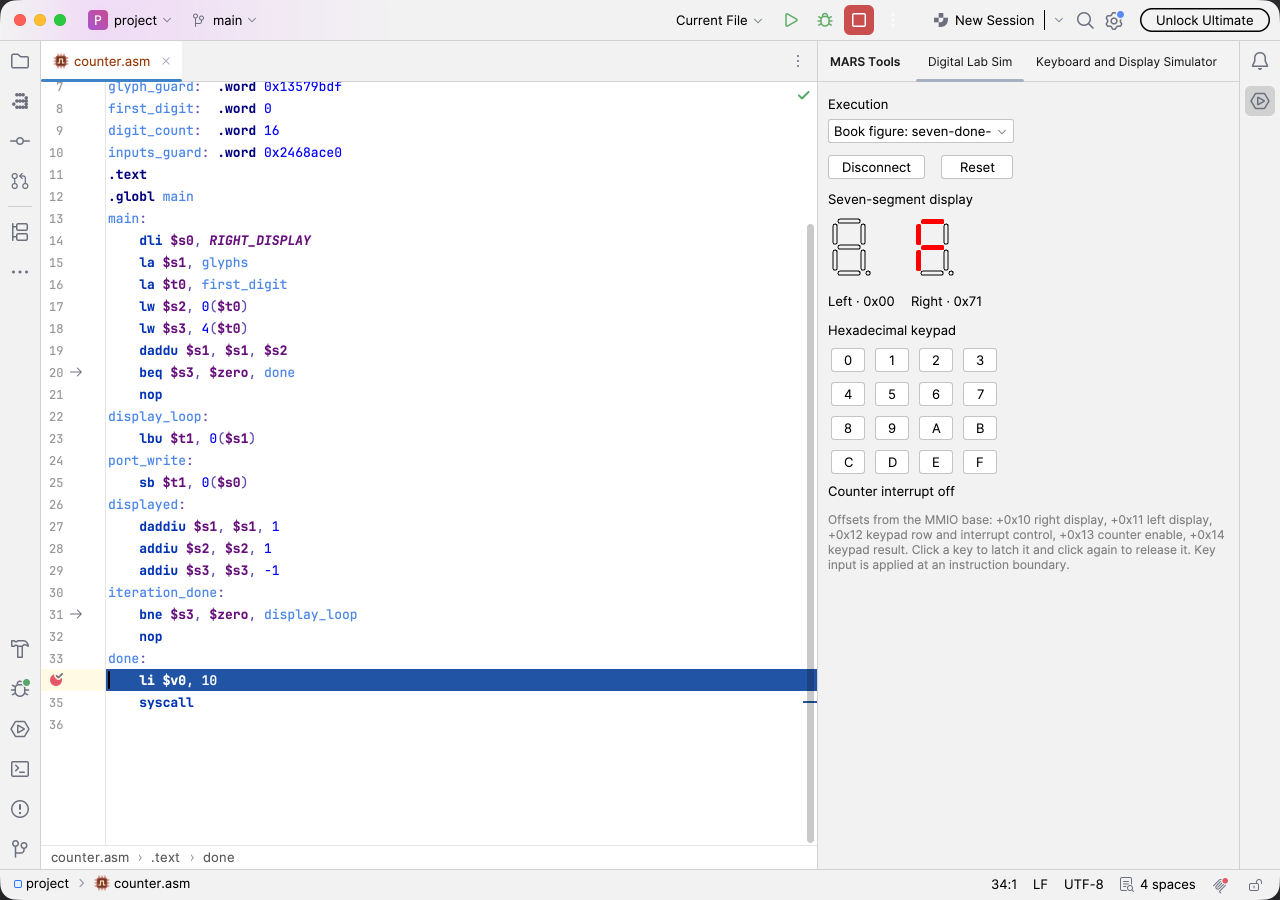
\includegraphics[width=0.34\linewidth,artifact,trim={\MARSfinallabLeft{} \MARSfinallabBottom{} \MARSfinallabRight{} \MARSfinallabTop{}},clip]{packages/005-seven-segment-counter/captures/f04-final-f/lab.png}};
\begin{scope}[shift={(lab.south west)},x={($(lab.south east)-(lab.south west)$)},y={($(lab.north west)-(lab.south west)$)}]
\draw[black,line width=0.7pt] (0.024539877,0.214876033) rectangle (0.815950920,0.818181818);
\node[draw=black,fill=white,circle,inner sep=1.5pt,font=\footnotesize] at ($(0.024539877,0.818181818)+(-3mm,0)$) {2};
\end{scope}
\node[anchor=north west,inner sep=0,font=\small\bfseries] (registers-title) at ([yshift=-2mm]lab.south west) {The next index is sixteen};
\node[anchor=north west,inner sep=0] (registers) at ([yshift=-1mm]registers-title.south west) {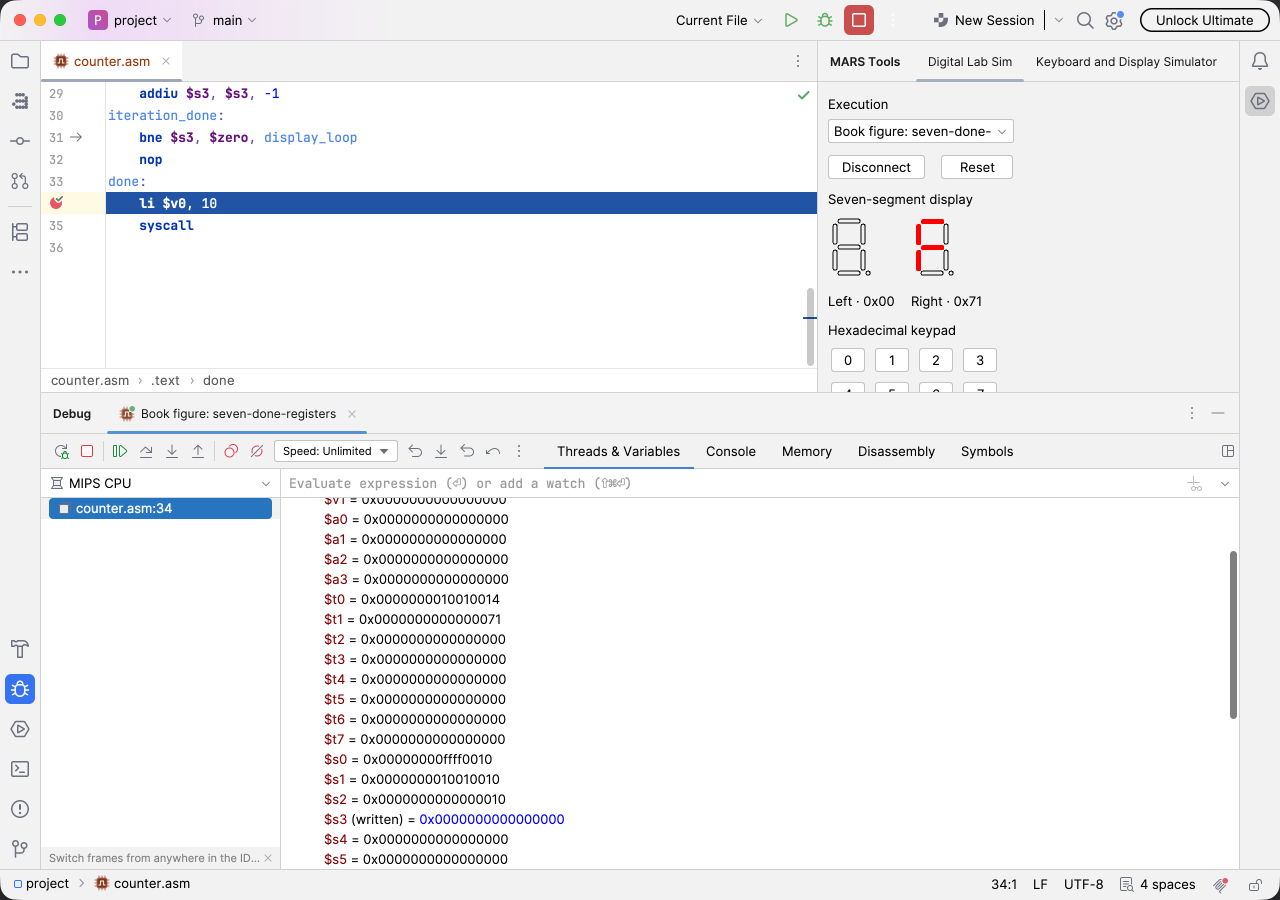
\includegraphics[width=0.43\linewidth,artifact,trim={\MARSfinalregistersLeft{} \MARSfinalregistersBottom{} \MARSfinalregistersRight{} \MARSfinalregistersTop{}},clip]{packages/005-seven-segment-counter/captures/f04-final-f/registers.png}};
\begin{scope}[shift={(registers.south west)},x={($(registers.south east)-(registers.south west)$)},y={($(registers.north west)-(registers.south west)$)}]
\draw[black,line width=0.7pt] (0.023346304,0.065217391) rectangle (0.976653696,0.934782609);
\node[draw=black,fill=white,circle,inner sep=1.5pt,font=\footnotesize] at ($(0.023346304,0.934782609)+(-3mm,0)$) {3};
\end{scope}
\node[anchor=north west,inner sep=0,font=\small\bfseries] (memory-title) at ([yshift=-2mm]registers.south west) {The source table and inputs remain unchanged};
\node[anchor=north west,inner sep=0] (memory) at ([yshift=-1mm]memory-title.south west) {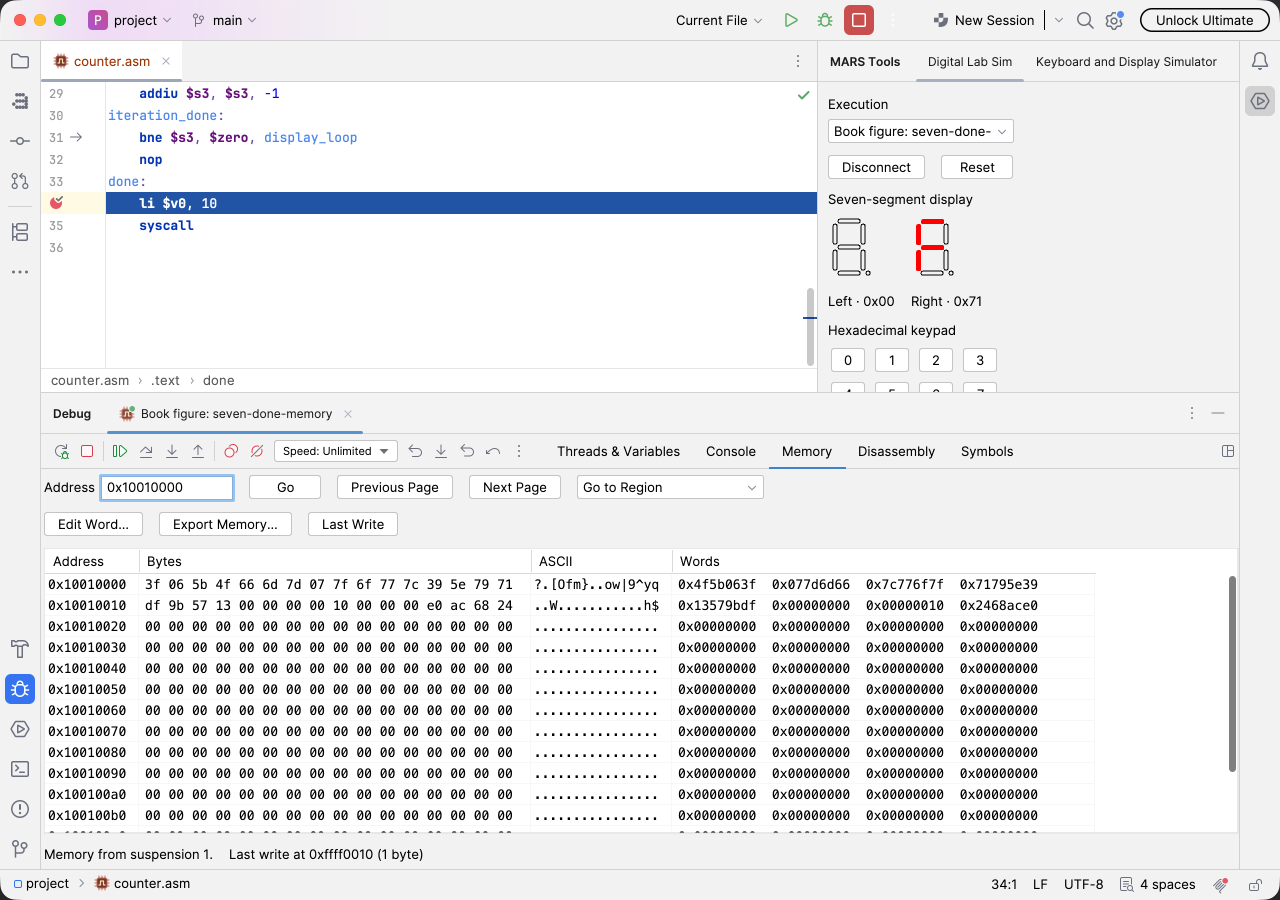
\includegraphics[width=0.84\linewidth,artifact,trim={\MARSfinalmemoryLeft{} \MARSfinalmemoryBottom{} \MARSfinalmemoryRight{} \MARSfinalmemoryTop{}},clip]{packages/005-seven-segment-counter/captures/f04-final-f/memory.png}};
\begin{scope}[shift={(memory.south west)},x={($(memory.south east)-(memory.south west)$)},y={($(memory.north west)-(memory.south west)$)}]
\draw[black,line width=0.7pt] (0.191919192,0.055555556) rectangle (0.983838384,0.638888889);
\node[draw=black,fill=white,circle,inner sep=1.5pt,font=\footnotesize] at ($(0.191919192,0.638888889)+(-3mm,0)$) {4};
\end{scope}
\end{tikzpicture}
\par\smallskip
\begin{minipage}{\linewidth}
\small
\begin{enumerate}
\item The next instruction, \texttt{li \$v0, 10}, begins the normal exit sequence. All sixteen iterations have completed, including the final pointer and counter updates. This stop is before the exit syscall.
\item The right mask \texttt{0x71} forms F; the left remains \texttt{0x00}. F was table entry fifteen. The tool retains the last byte written, so the completed loop does not blank the display. Both decimal points remain off.
\item \texttt{\$s2}=\texttt{0x10}=16 is now the next index, beyond the last entry used. \texttt{\$s3}=0 ends the loop. Neither value is the current display mask. No further table load or display store is needed.
\item The first row retains all sixteen glyph bytes, ending in \texttt{71}. The next row retains guard \texttt{0x13579bdf}, first index 0, count 16 and guard \texttt{0x2468ace0}, each as four little-endian bytes. The transaction check also rejects temporary writes later restored to these values. All sixteen output transactions must be byte stores to the fixed right port.
\end{enumerate}
\end{minipage}
\caption{The default range is complete before the exit sequence. The display retains F while the counters describe the end of the range.}
\label{capture:005-seven-segment-counter-f04-final-f}
\end{figure}
\par
